% Created 2023-10-13 Fri 17:45
% Intended LaTeX compiler: pdflatex
\documentclass[11pt]{article}
\usepackage[utf8]{inputenc}
\usepackage[T1]{fontenc}
\usepackage{graphicx}
\usepackage{longtable}
\usepackage{wrapfig}
\usepackage{rotating}
\usepackage[normalem]{ulem}
\usepackage{amsmath}
\usepackage{amssymb}
\usepackage{capt-of}
\usepackage{hyperref}
\usepackage{placeins}
\usepackage{gensymb}
\author{Christian}
\date{\today}
\title{}
\hypersetup{
 pdfauthor={Christian},
 pdftitle={},
 pdfkeywords={},
 pdfsubject={},
 pdfcreator={Emacs 28.2.50 (Org mode 9.7-pre)}, 
 pdflang={English}}
\begin{document}

\tableofcontents

\section{Problem 1}
\label{sec:orgaf1f1e2}
\subsubsection{A. Design a Butterworth LOW PASS filter}
\label{sec:org92a1ed8}
\begin{enumerate}
\item Specifications:
\label{sec:orgbe4fcbe}
\begin{itemize}
\item DC Gain = 0 dB
\item Amax = 1.0 dB
\item Amin = 30 dB
\item ωp = 2000 rad/sec
\item ωs = 4700 rad/sec
\end{itemize}
Use Case 2 Sallen-Key circuit(s) (Figure 4.8) with R = 10kΩ
\item My Work
\label{sec:orge4674f1}
\begin{center}
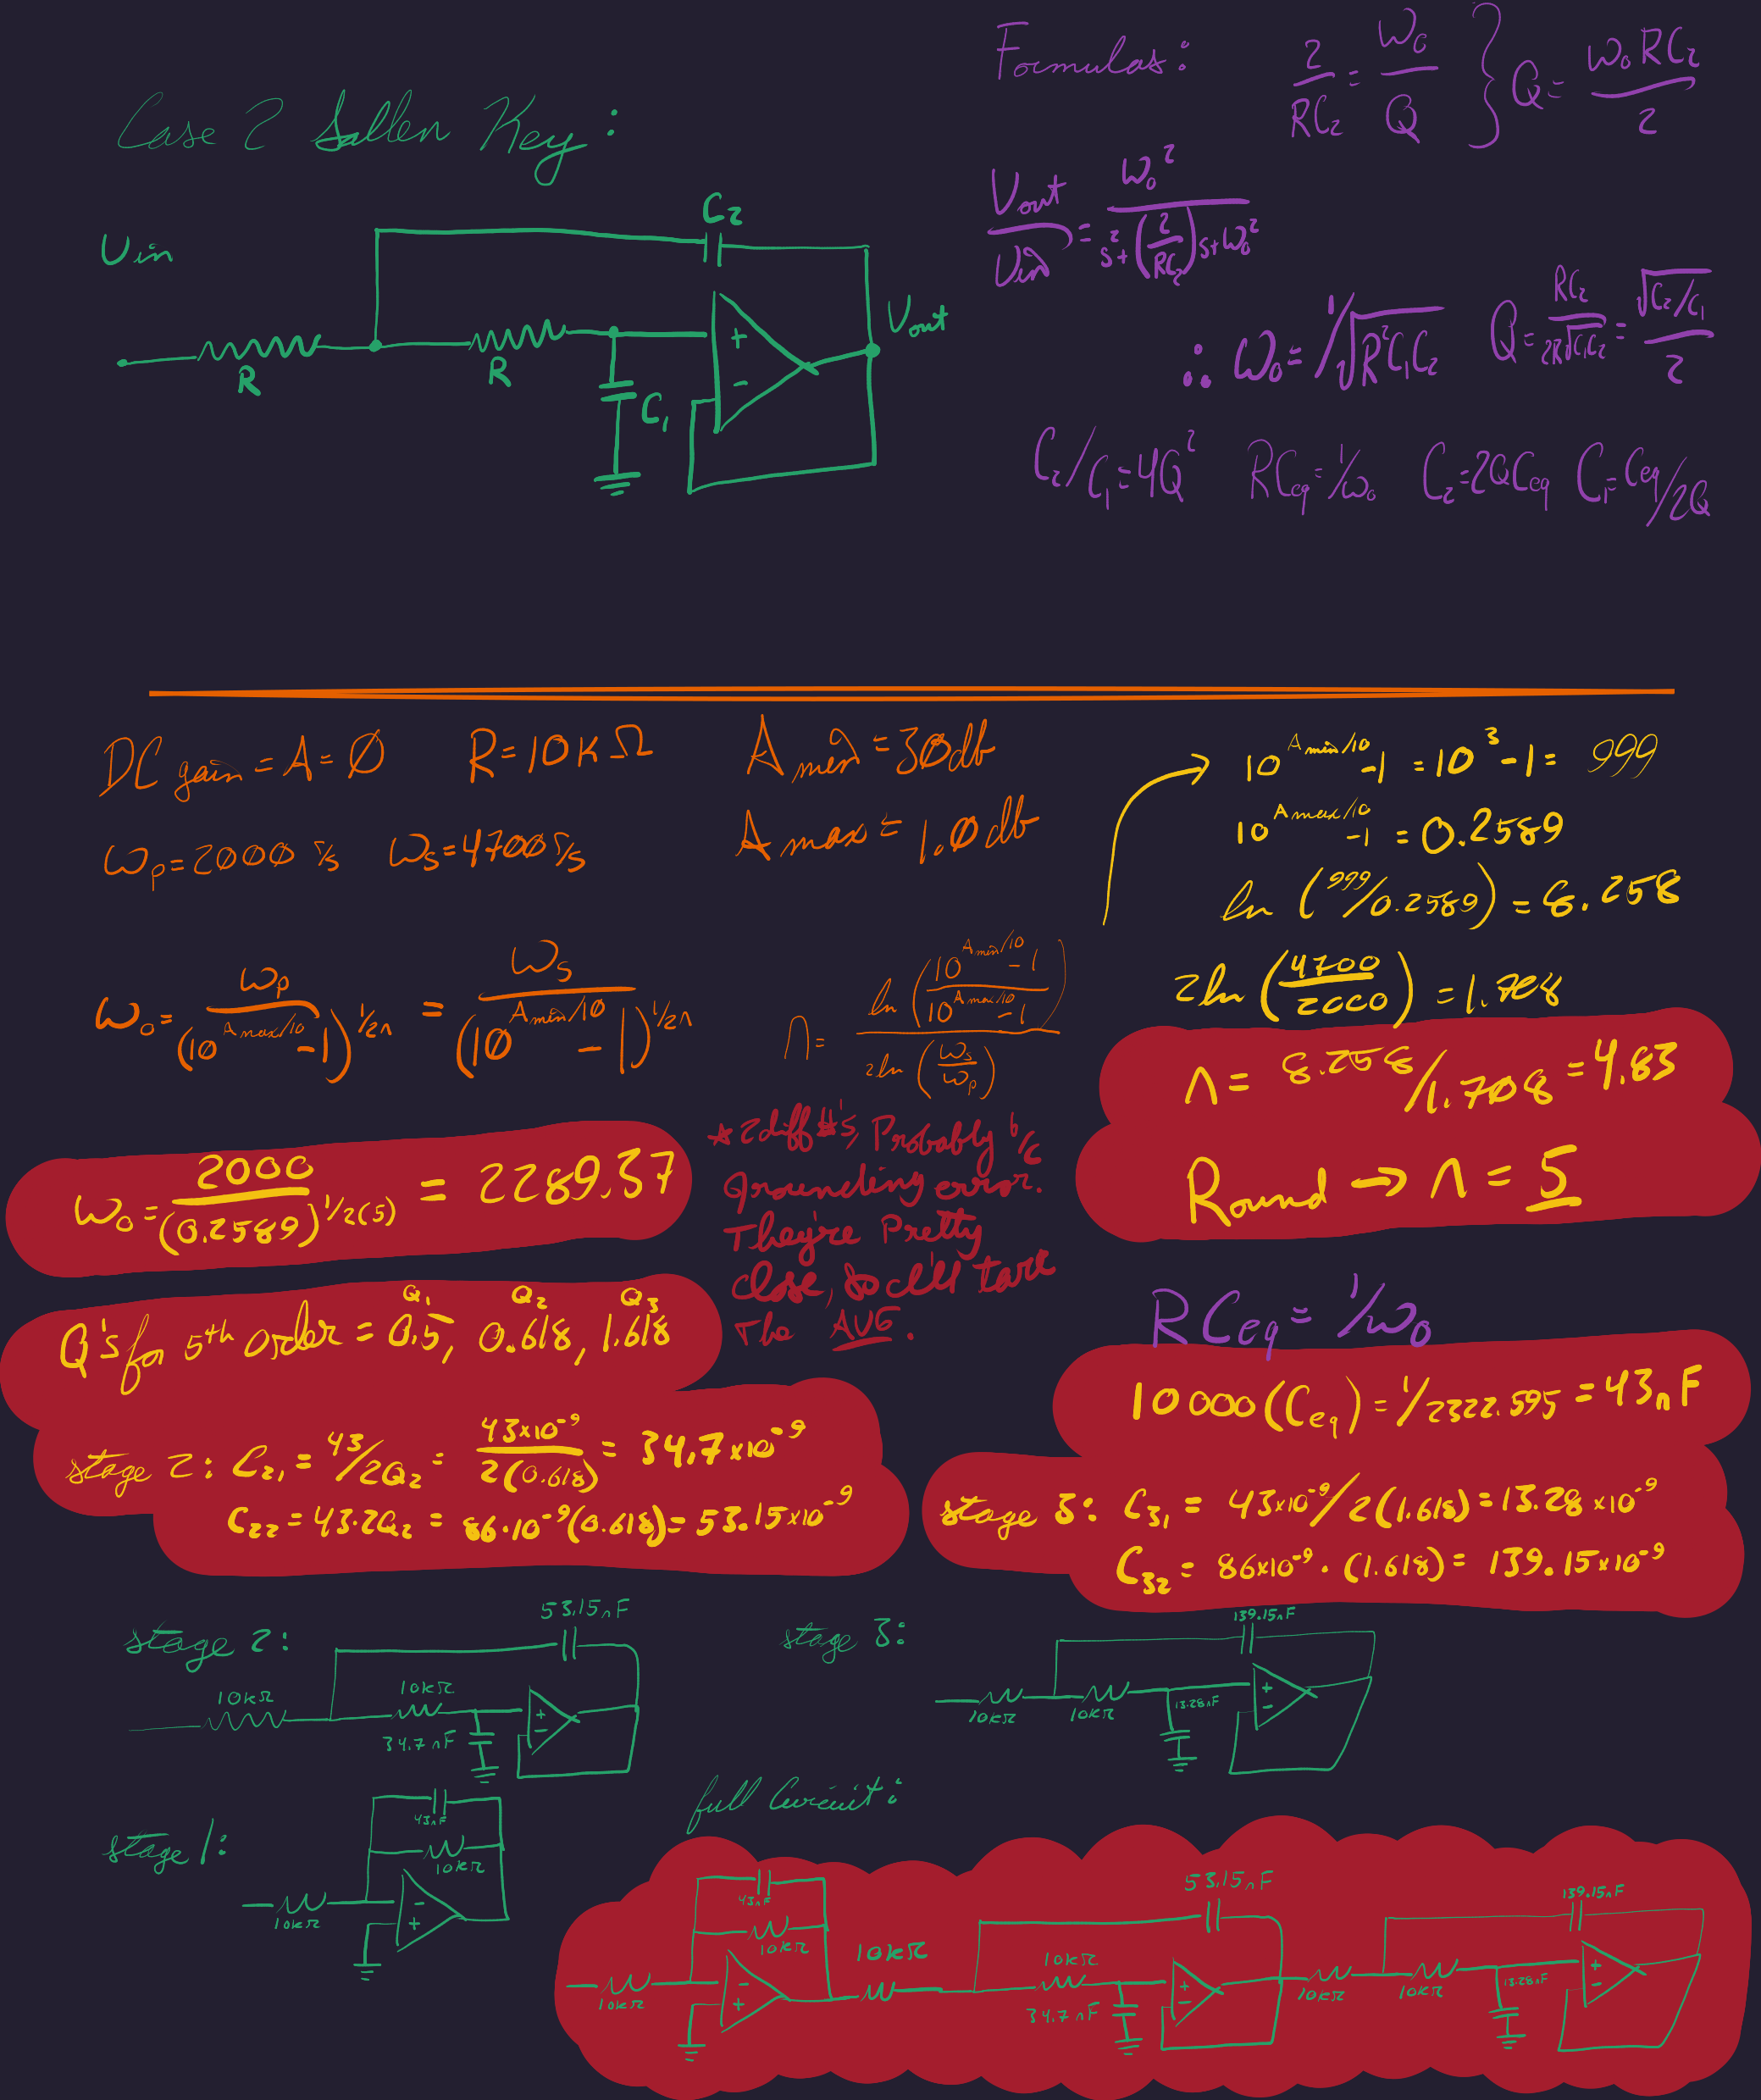
\includegraphics[width=.9\linewidth]{/home/csj7701/class/F23/Linear/Homework/Homework5-1.png}
\end{center}
\end{enumerate}
\subsubsection{B. Matlab Plot}
\label{sec:org79528de}
Plot the MAGNITUDE response for each section of your design and the overall MAGNITUDE response.

\begin{verbatim}
%Problem#1
wo1=2289.37;Q1=0.5;
wo2=2289.37;Q2=0.618;
wo3=2289.37;Q3=1.618;
Num1=wo1;
Num2=wo2^2;
Num3=wo3^2;
Den1=[1 wo1];
Den2=[1 wo2/Q2 wo2^2];
Den3=[1 wo3/Q3 wo3^2];
w=logspace(2,4,1000);
H1=freqs(Num1,Den1,w);
H2=freqs(Num2,Den2,w);
H3=freqs(Num3,Den3,w);
H=H1.*H2.*H3;
H1db=20*log10(abs(H1));
H2db=20*log10(abs(H2));
H3db=20*log10(abs(H3));
Hdb=20*log10(abs(H));
semilogx(w,Hdb,w,H1db,w,H2db,w,H3db);
grid;xlabel('frequency in rad/sec');ylabel('Magnitude (dB)')
title('Magnitude Response Problem#1');
\end{verbatim}

\begin{center}
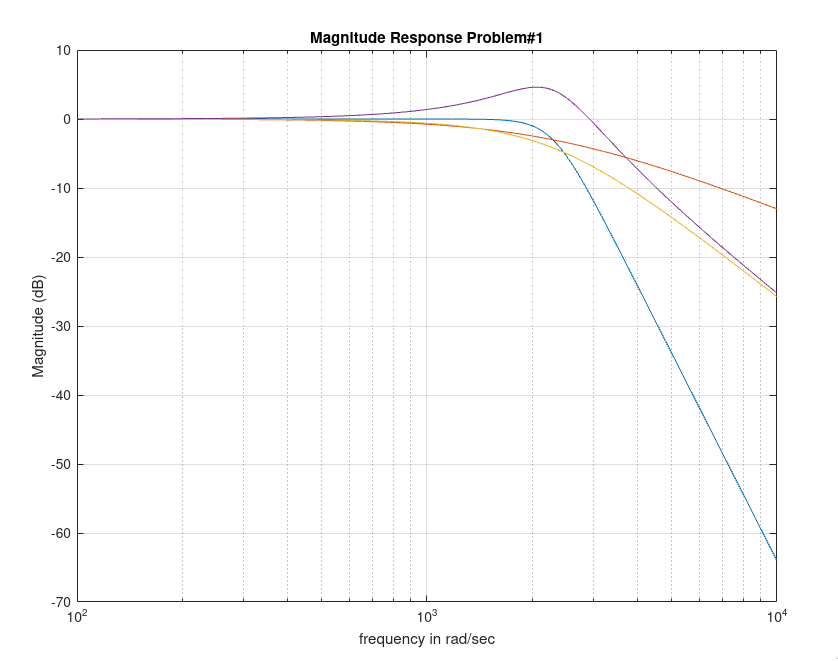
\includegraphics[width=.9\linewidth]{/home/csj7701/class/F23/Linear/Homework/Mag-1.png}
\end{center}
\section{Problem 2}
\label{sec:orgff93135}
\subsubsection{A. Design a Butterworth LOW PASS filter}
\label{sec:orge388456}
\begin{enumerate}
\item Specifications:
\label{sec:org3eece12}
\begin{itemize}
\item DC Gain = 4 dB
\item Amax = 2 dB
\item Amin = 25 dB
\item ωp = 6000 rad/sec
\item ωs = 14000 rad/sec
\end{itemize}
Use Case 1 Sallen-Key circuit(s) and a voltage divider with R = 10kΩ
\textbf{NOTE} each stage will have a gain of \(A=1+\frac{R_{b}}{R_{a}} = 3-\frac{1}{Q}\), which means we need a voltage divider. (Probably only one).
\item My work
\label{sec:orgdfd716b}
\begin{center}
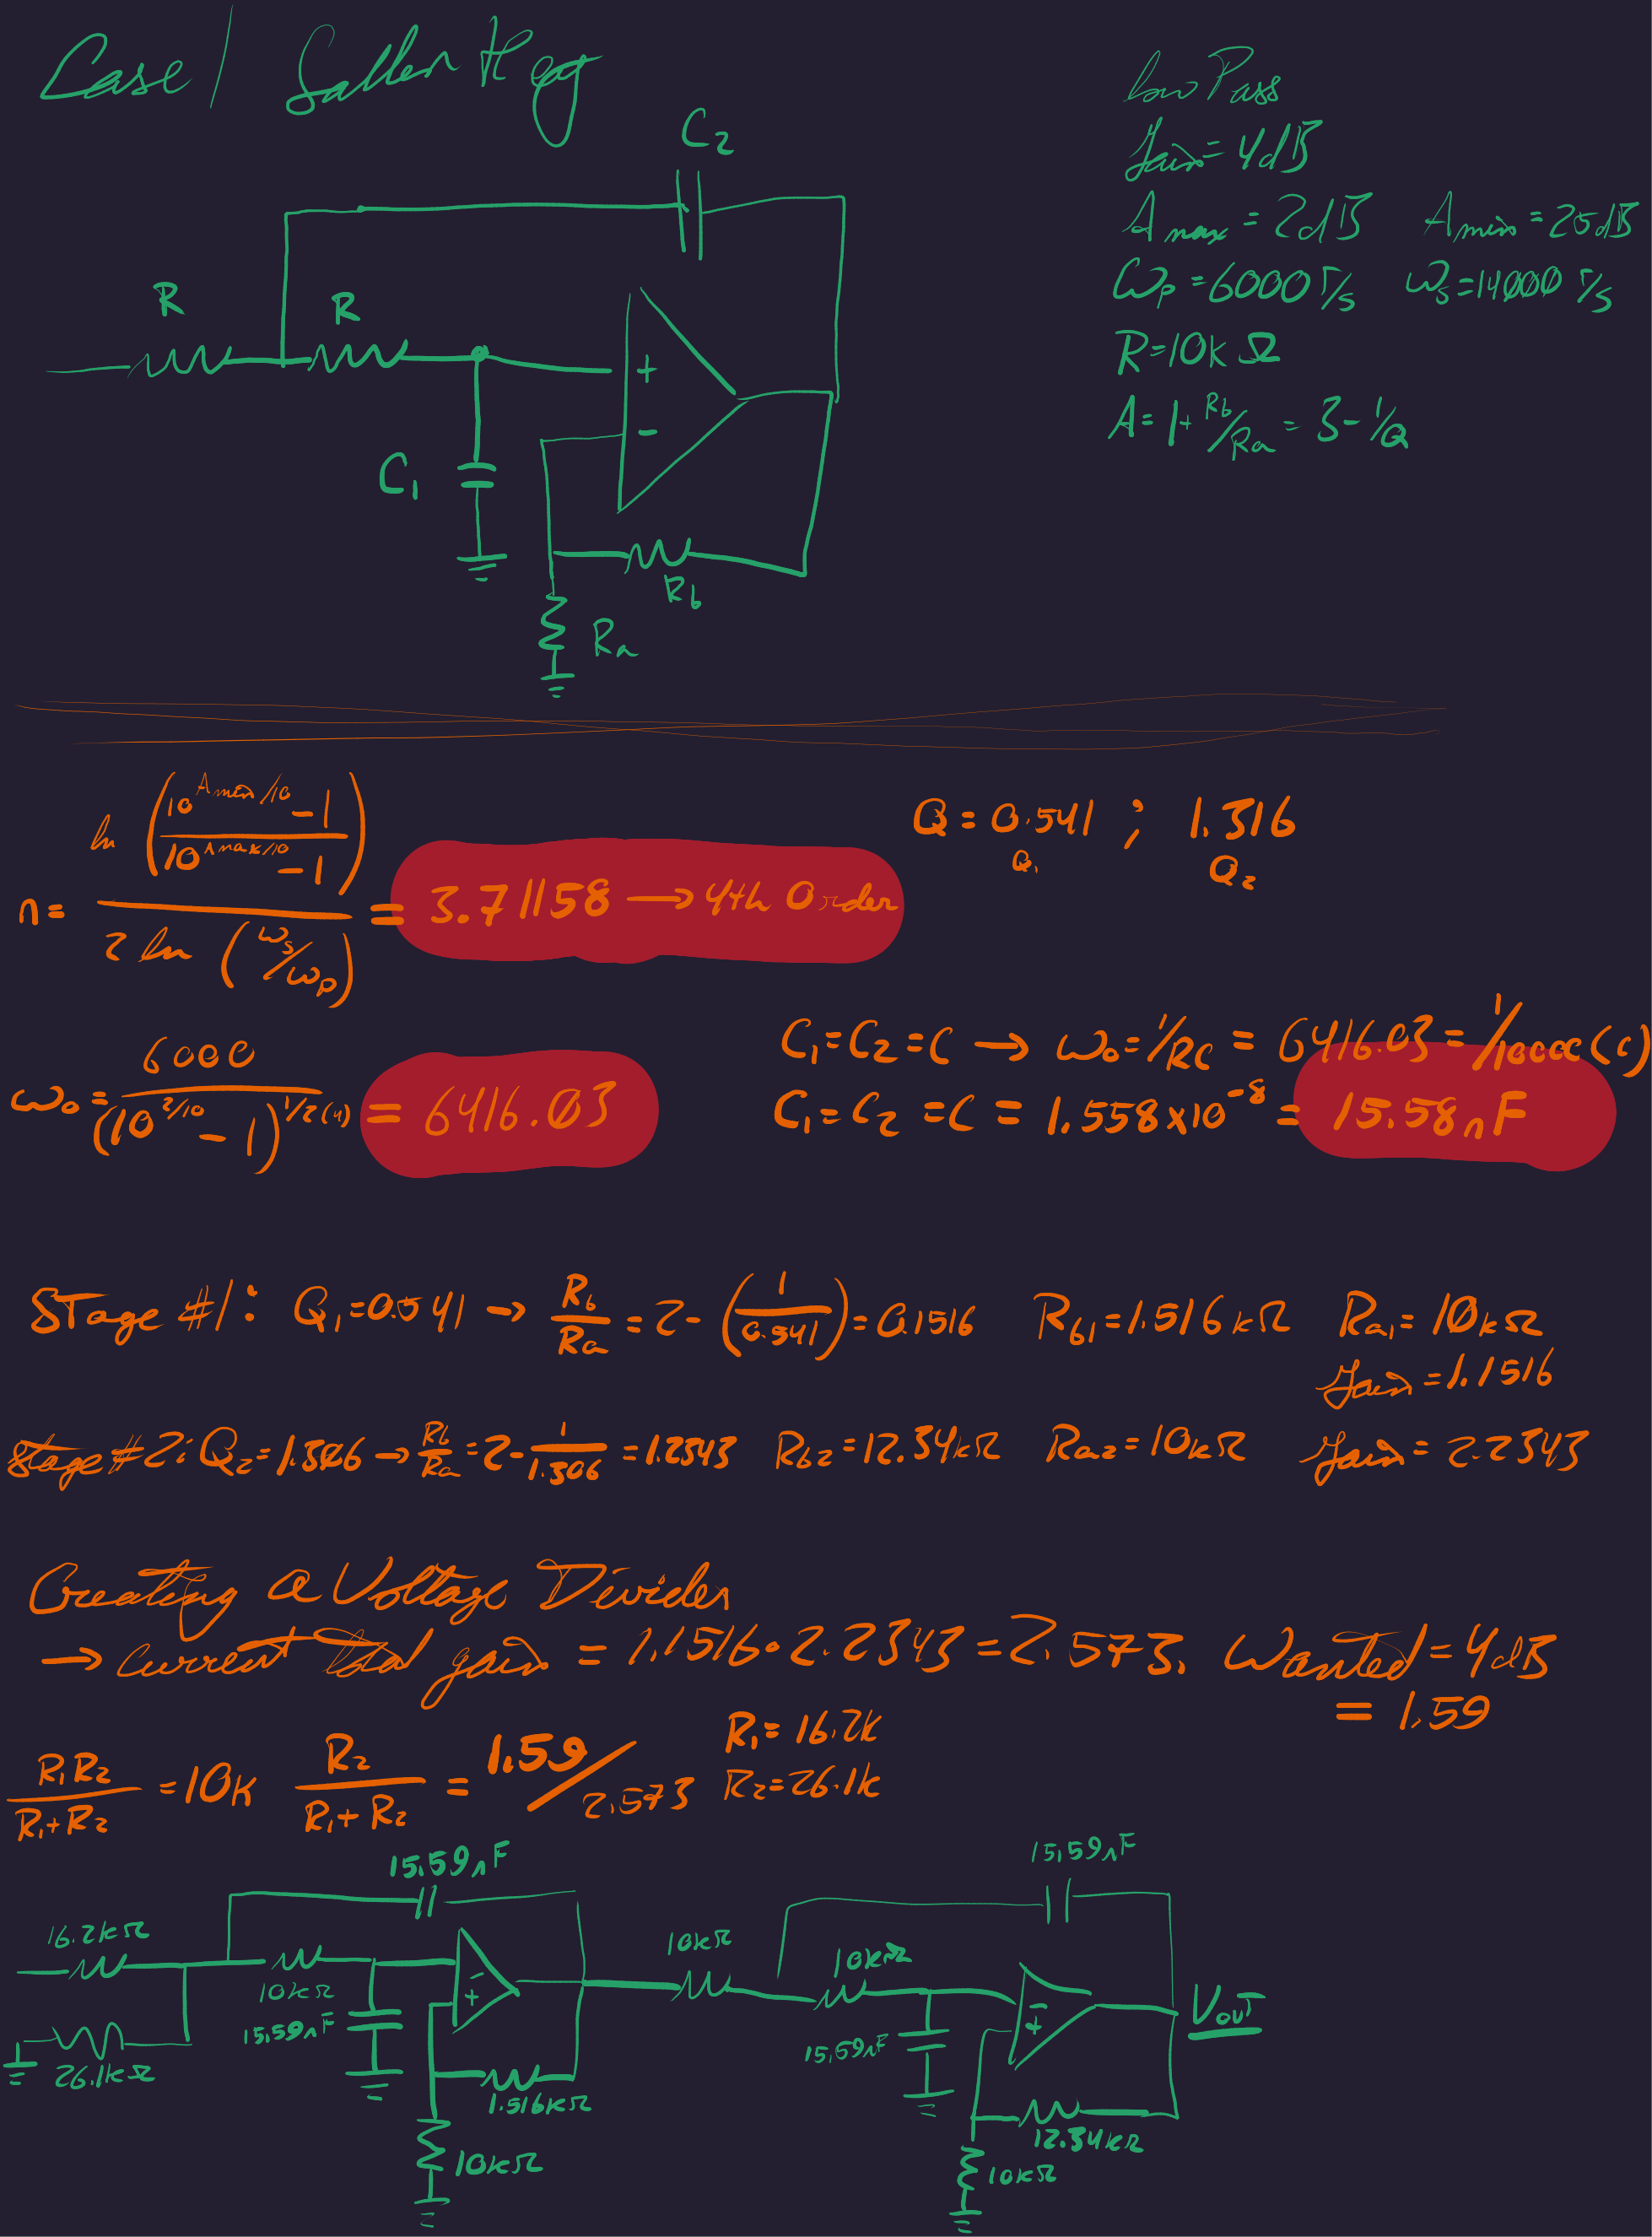
\includegraphics[width=.9\linewidth]{/home/csj7701/class/F23/Linear/Homework/Homework5-2.png}
\end{center}
\end{enumerate}
\subsubsection{B. Matlab Plot}
\label{sec:orgee79ec4}
Plot the MAGNITUDE response for each section of your design and the overall MAGNITUDE response.
\begin{center}
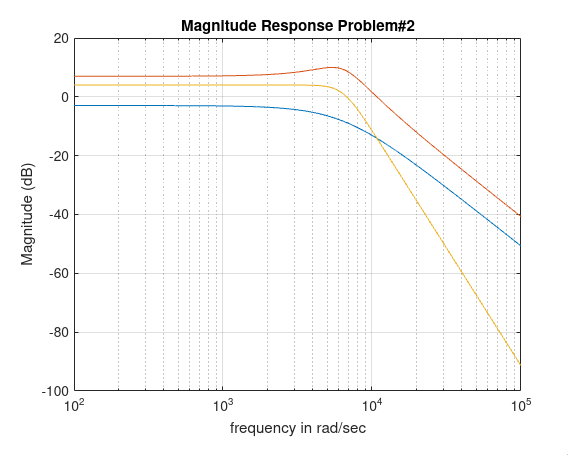
\includegraphics[width=.9\linewidth]{/home/csj7701/class/F23/Linear/Homework/Mag-2.png}
\end{center}
\section{Problem 3}
\label{sec:org6703505}
\subsubsection{A. Design a Butterworth HIGH PASS filter}
\label{sec:org30b8fe0}
\begin{enumerate}
\item Specifications:
\label{sec:org062f205}
Design for Problem 4.17 in your textbook
Use Case 1 Sallen-Key circuit and design equations (4.53) and (4.54)
You should require a 4th order filter to meet this specification
Use ONE voltage divider (a capacitive voltage divider!) at the beginning of the 1st stage to set your overall DC Gain to 0dB. Use R = 10kΩ where possible in your design.
\item My work
\label{sec:orgc0e2212}
\begin{center}
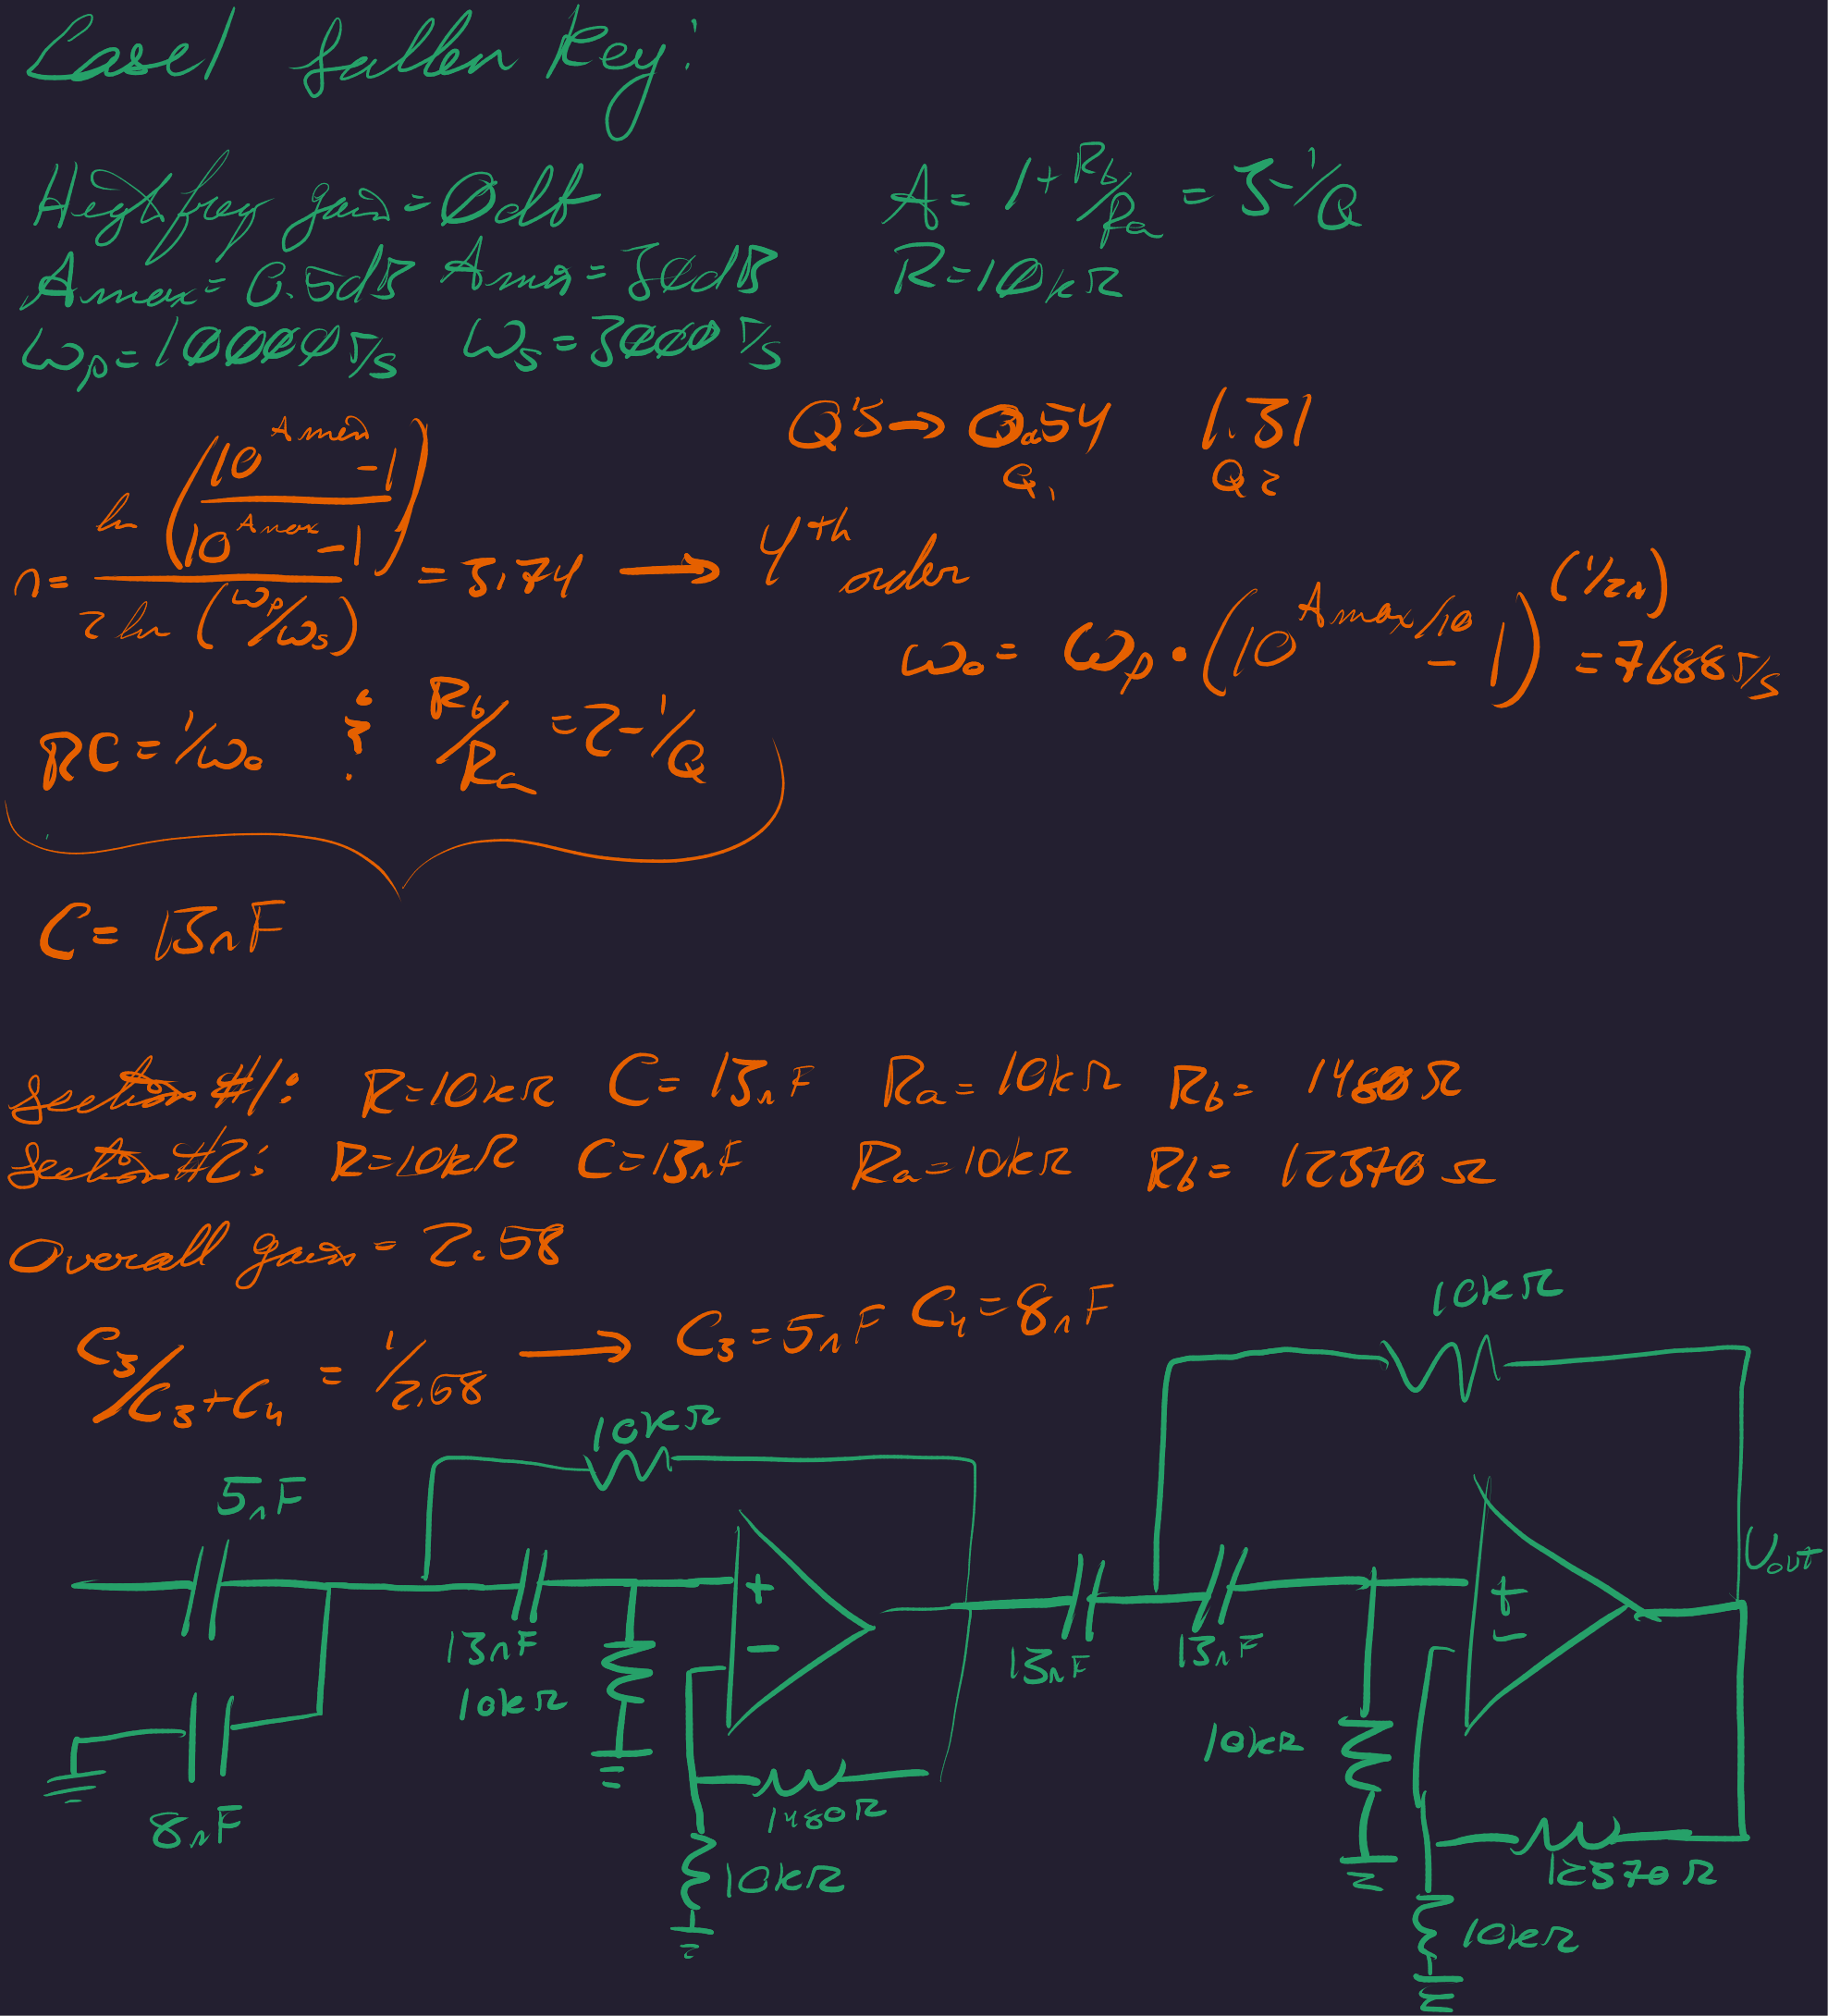
\includegraphics[width=.9\linewidth]{/home/csj7701/class/F23/Linear/Homework/Homework5-3.png}
\end{center}
\end{enumerate}
\subsubsection{B. Matlab Plot}
\label{sec:orga9402b8}
Plot the MAGNITUDE response for each section of your design and the overall MAGNITUDE response.
\begin{center}
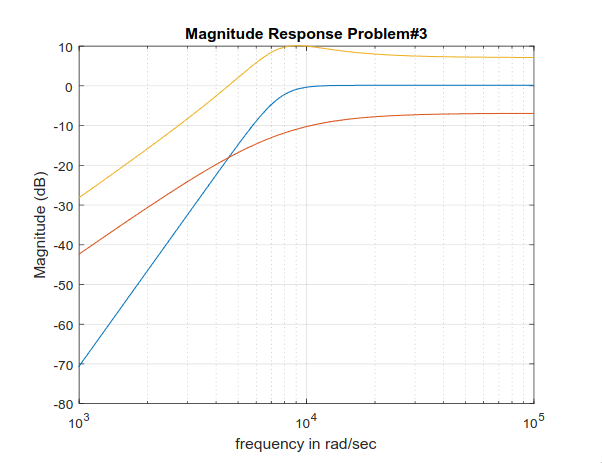
\includegraphics[width=.9\linewidth]{/home/csj7701/class/F23/Linear/Homework/Mag-3.png}
\end{center}
\section{Problem 4}
\label{sec:org0e622ef}
Write a MATLAB function to calculate the pole locations for a Butterworth low pass filter, given filter specifications.
\begin{verbatim}
function[poles] = CJ_Butterpoles(n,w)
    k=0:(2*n-1);
    if(mod(n,2)==1)
        poles=w*exp(j*2*pi*k/(2*n));
    else
        poles=w*exp(j*(2*k+1)*pi/(2*n));
    end
    poles=poles(real(poles)<0);
    return
\end{verbatim}
\section{Problem 5}
\label{sec:orge2e17a8}
Write a MATLAB function to display Wo’s and Q’s associated with a set of poles.
\begin{verbatim}
function[] = CJ_QWgraph(poles)
% Function Name: Display_Wos_and_Qs
%% Parameters: Poles (get passed in)
% Returns: dummy (i.e. nothing)
% Description: Displays Wo's and Q's for any set of poles
    Q = (1./(2*cos(angle(poles))));
    numpoles = length(poles);
    k = 0:numpoles-1;
    wo = zeros(size(k));
    if (mod(numpoles,2)==1)
        for i = 1:length(k)
            wo(i) = poles(i)/exp(1j*k(i)*pi/numpoles)
        end
    else
        for i = 1:length(k)
            wo(i) = poles(i)/exp((1j*(2*k(i)+1)*pi)/(2*numpoles))
        end
    end
    polarplot(poles,'o');
    return;
end
\end{verbatim}
\end{document}